\chapter{Implementation}
\section{Requirements and Goals}
Depending upon the function we can split the design of a PMU in three parts. 
A. Signal Input \& Sampling part
B. Processing of Samples  
C. Transmission of data
Here different parts will have different requirements. So, we will first state the minimum requirement stated by standards or aimed by us.

\begin{enumerate}
	\item \textbf{ADC Requirements}
	While deciding upon the ADC specification we kept following requirements: 
	\begin{itemize}
		\item Good sampling rate: ~64 Samples/cycle
		\item No of channels: 3 + 3 = 6 (3 - $\phi$ voltage and current) 
		\item Interfacing type: It should be memory addressable and voltage level compatible .
		\item Input type: FSS analog output is differential which can be configured as single ended, it's voltage level is $\pm$10V
	\end{itemize}
	
	\item \textbf{Processing Requirements}
	PMU has stringent timing requirement, samples needs to be processed in given deadline of reporting time, for this a processor having good ALU would be preferable, for which DSP core is best suited for rapid low level and hard realtime computation. Normal Discrete Fourier Transform requires of complexity O($N^{2}$) operations hence the computation requirement increases as the sample count increases. 
	
	\item \textbf{Data Transmission Requirements }
	Realtime transmission of data is mandated by the standards \cite{c37.118}. For that different protocols like Realtime  Media Transfer Protocol (RMTP) or other ways can be used but it would require a sufficiently capable ethernet socket, so we decided to have at least 10/100 MBPs.
	
\end{enumerate}

\section{BeagleBone Black}
Initially we decided to use TI OMAPL-137 which is a dual asymmetric-core processor, in which one core is of DSP and other one is of ARMv7 a brief description is given in Appendix. Due to a mishap our OMAP L137 stopped working so new processor was chosen. which was AM3359 which is a single core ARM Cortex-A8, 1 GHz processor, we decided to use BeagleBone Black which is an low-coast open source community supported multipurpose board. All hardware design is made available and complete programmatic access to the hardware is given which gives complete flexibility for development and implementation. Simplified technical description of the board is given below:
\begin{table}[h]
		\begin{center}
			\setlength\arrayrulewidth{1pt}
			\begin{tabular}{|c|c|}
				\hline
				Processor & Sitara AM3358BZC 1 GHz, 2000MIPS\\
				\hline
				Graphic Engine  SGX530 3D, 20M & Polygons/S\\
				\hline
				SDRAM Mem & 512 MB DDR3L 800MHz \\
				\hline
				Onboard Flash 4GB, 8-bit Embedded MMC \\
				\hline
				Serial Port & UART0-4 via 6 pin header 3.3V TTL\\ 
				\hline
				HS USB 2.0 Client ports & USB0 access to client via mini-USB\\
				\hline
				HS USB 2.0 Host Port & Type -A Socket 500mA \\
				\hline
				Ethernet & 10/100, RJ45 \\
				\hline
				SD/MMC Connector & microSD, 3.3 V\\
				\hline
				Video Output & 16b HGMI, 1280x1024 (MAX)\\
				\hline 
				\multirow{3}{10pt}{Expansion Connectors} & power 5v, 3.3V, VDD\_ADC (1.8v) GPIO(69 Pins), LCD, GPMC, MMC1 MMC2 7 ADC in-pins	XDMA Interrupt,
				Power button, Expansion Board ID\\
				\hline
				
			\end{tabular}
		\end{center}
\end{table}

As we can see, specification are pretty impressive but the most important feature of this board are the PRU-ICSS, Programmable Realtime Units Industrial Communication subsystems. Which are two independent 200Mhz 32bit RISC cores . They operate completely independent from the the ARM core,  allowing independent operation and clocking for greater efficiency and flexibility. The PRU-ICSS enables additional peripheral interfaces and real-time protocols. In addition they have fixed execution time, they are connected to (almost) all peripherals with Enhanced Data Bus for (for GPIO for) better communication. PRUs can be programmed separately by loading them with a binary file. Brief description of PRUs are given below

\subsection{PRU Subsystem}
The Programmable Real-Time Unit Subsystem and Industrial Communication Subsystem (PRU-ICSS) consists of dual 32-bit RISC cores (Programmable Real-Time Units, or PRUs), shared, data, and instruction memories, internal peripheral modules, and an interrupt controller (INTC). The programmable nature of the PRU, along with its access to pins, events and all SoC resources, provides flexibility in implementing fast real-time responses, specialized data handling operations, custom peripheral interfaces, and in offloading tasks from the other processor cores of the system-on-chip (SoC).

\begin{figure}
	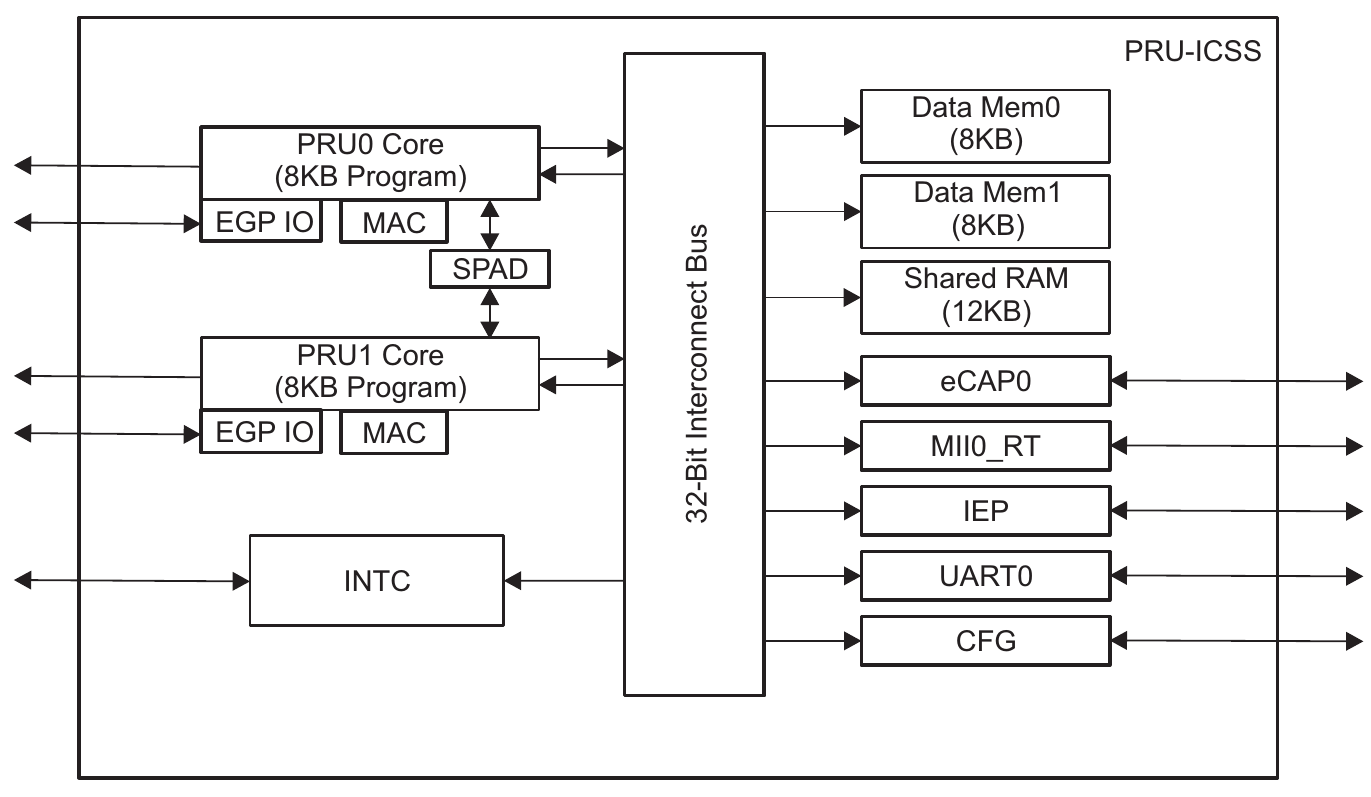
\includegraphics[width=\textwidth]{fig/PRUIcss.png}
	\caption{Block Diagram of PRU Subsystem}
	\label{fig:prublkdrg}
\end{figure}

Useful features that we are using and are worth noting are as follow:
\begin{itemize}
	\item Two PRUs each with:
	\begin{itemize}
		\item 8KB program memory
		\item 8KB data memory
		\item High Performance Interface/OCP Master port for accessing external memories
		\item Enhanced GPIO (EGPIO) with async capture and serial support
		\item Multiplier with optional accumulation (MPY/MAC)		
	\end{itemize}
	\item scratch pad (SPAD) memory with 3 banks of 30, 32-bit registers 
	\item Broadside direct connect between PRU cores within subsystem
	\item 12 KB general purpose shared memory
	\item One Interrupt Controller
	\item One 16550-compatible UART with a dedicated 192-MHz clock.
\end{itemize} 

\subsection{ADC Subsystem}
AM3358 has 200ksps 8 channel muxed single SAR type ADC on it. It is important to understand the functioning of ADC system because we are using few specific features in our implementations (viz Steps, Open Delay and Sample Delay). AM3358 has Touch Screen Controller and Analog to Digital Converter system combined (know as TSC\_ADC\_Subsystem) \cite{AM3358TRM} . Few main feature of ADC Systems are: 
\begin{itemize}
	\item[--] Programmable FSM sequencer that supports 16 steps.
	\item[--] Software register bit for start of conversion
	\item[--] Dual Conversion Modes: One-shot \& Continuous
	\item[--] Sequence through all input channels based on a mask
	\item[--] Programmable OpenDelay before sampling each channel
	\item[--] Programmable sampling delay for each channel
	\item[--] Programmable averaging of input samples - 16/8/4/2/1
	\item[--] Differential or singled ended mode setting for each channel
	\item[--] Store data in either of two FIFO groups
	\item[--] Dynamically enable or disable channel inputs during operation
\end{itemize}
AM3358's ADC system is very flexible and hence bit complicated to use. Each function is controlled by a ``step" so each activated feature (either ADC or TSC) is assigned a step number between 1-15 (step -0 is charge step, for touch screen; Step-16 idle) and accordingly the sequencer will iterate through the steps and there by channel(s). sequencer is completely software controlled so the sampling trigger or delay can be configured programmatically.
\begin{itemize}
	\item \textbf{Open Delay \& Sample Delay:} User can decide when the voltage should be driven to the ADC and when should ADC start sampling. This delay is used for letting the voltage stabilize in case of weak signal input or impedance mismatch.This is \textit{Open Delay}. Sample Delay decides the width of the SoC width.
	\item \textbf{Averaging of Sample:} ADC system has an averaging system which averages 1(no averaging), 2, 6 ,8 12 and 16 times. If averaging is tunrned ON, say for N samples then ADC system will immediately re-sample the signal (same channel) N times, will average all the samples \textit{and then} will put it to FIFO buffer.
	\item \textbf{Single-Shot or Continuous Mode:} In Oneshot mode sequencer finishes the sampling and conversion of all enabled channels, disables the channels and waits for another trigger. In continuous mode, sequencer loops back to the first step to restart the conversion process all over again, till the STEPENABLE bit is resetted.    
\end{itemize} 

\section{Implementation Overview}
An overview of PMU implementation, using AM335x based BeagleBone Black is show in fig 
\begin{figure}
	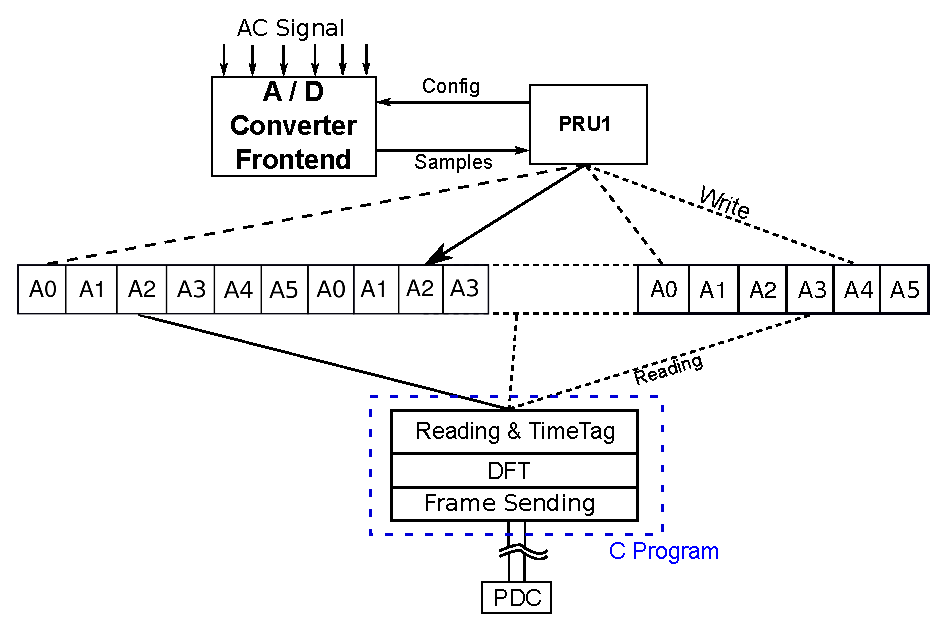
\includegraphics[width=\textwidth]{fig/sys_overview.eps}
	\caption{Overview of implementation}
\end{figure}

The implementation being described is a synchronized operation of three independent asynchronous subsystems: PRU, ADC and ARM core.
\begin{itemize}
	\item A C program is written which configures PRU and uploads a binary file in to the PRU(1). PRU binary files does three task:
	\begin{enumerate}
		\item Configure ADC, with 
		\begin{itemize}
			\item Enables 6 channels by writing to \texttt{STEPCONFIGx}
			\item Configures Open Delay (\texttt{OpD}) = 0, by writing zeros to \texttt{STEPDELAYx} register  
			\item Sample delay (\texttt{SaD}) = 0 
			\item Sample Averaging (\texttt{SAvg}) = 1  by writting ones to  \texttt{STEPCONFIGx} registers and 
			\item Timer delay [\texttt{Tmr}]= 156250 ns
			\item \texttt{Mode} = continuous 
		\end{itemize}
		\item Define the bank to be used as buffer, and size of buffer
		\item Parse the data received from FIFO buffer (of ADC) in to the ring buffer. 
	\end{enumerate}
	\item 6 ADC channels are enabled and the sampling rate is set to 128 samples/cycle/channel (using \texttt{Tmr} delay). the OpenDelay and Sample Delay are kept zero because our signal strength is enough. Timer delay is configured to $ \frac{1}{128 * 50} = 156250 ~ns $.
	\item In continuous mode the buffer is defined as ring buffer and the   buffer length is kept $ 128 * 6 = 768 * 2 = 1536 $. buffer length is kept double for reading and filling the buffer in Ping-Pong fashion.  
	\begin{figure}[h]
		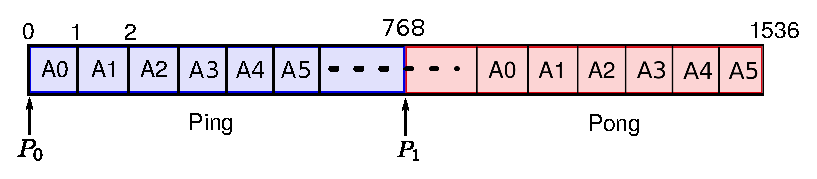
\includegraphics[width=\textwidth]{fig/ring_buffer.eps}
		\caption{Ring Buffer length and Ping Pong depicted}
		\label{fig:rb_pp}
	\end{figure}
	\item C program after uploading the bin file, sets the execution bit, This initiates the PRU execution, which signals ADC to start sampling with given configuration. PRU continuously fetches the the data from the output FIFO register of ADC and puts it in to ring buffer \textit{continuously} in sequential order of enabled channels [ \texttt{A0 A1 A2 A3 A4 A5 A0 A1.....A4, A5}].
	\item On the ARM side C program creates two pointers and using Ping Pong method over ring buffer reads the ADC samples in chunks. Brief description of how this works is described below and see Fig: \ref{fig:ping_pong}.
	\begin{itemize}
		\item[--] A buffer of double size then the target size is created (here of 1536 words) and two pointer  \texttt{P0} and \texttt{P1} are created, which points to the start and the middle of the buffer respectively. [ Step - 1 ]
		\item[--] Out of two pointer one works as \texttt{write head} and other as \texttt{read head}. So P0 keeps the track of number of ADC samples parsed in the buffer. [ Step-2 ]
		
		
		\begin{figure}
			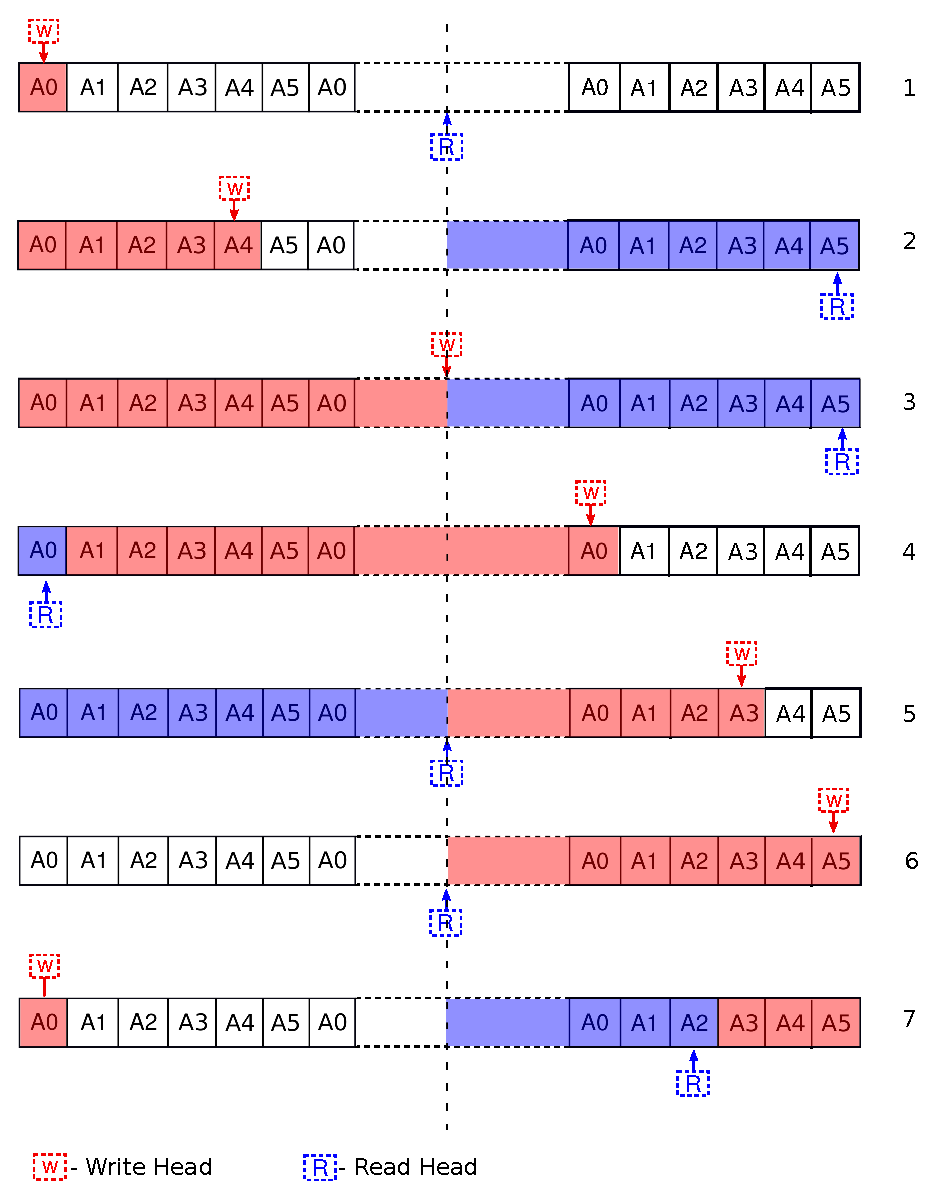
\includegraphics[width=\textwidth]{fig/ping_pong.eps}
			\caption{Ping-Pong Process Visualized}
			\label{fig:ping_pong}
		\end{figure}
		
		
		\item When P0 (write head) reaches 768 samples (128* 6, one whole cycle of all channels), pointers are swapped, P1 becomes the write head and P0 becomes the read head and goes to the beginning of the buffer and starts reading, while write head (pointer P1) continuous to write samples into buffer [ Step-3 ]
		\item Read operation is faster then write ( as PRU has to wait for the samples to arrive depending upon the sampling rate). read head reaches the middle while P1is still writing the samples. [ Step-5 ]
		\item After reaching the end of buffer, Pointers are again swapped, P1 again becomes the read head and P0 Write head, which starts reading from the middle and the write goes to the beginning of the buffer and starts filling the samples. [ Step-6 ]
		\item From this point it is same as the beginning and the whole cycle repeats. [ Step-7 ]
	\end{itemize} 
	\item This way C program keeps on toggling between two buffers and there by allowing for concurrent reading and writing operation
	\item A visual depiction of the Ping-Pong process described above is show in the Fig: \ref{fig:ping_pong}
\end{itemize}

\begin{figure}[h]
	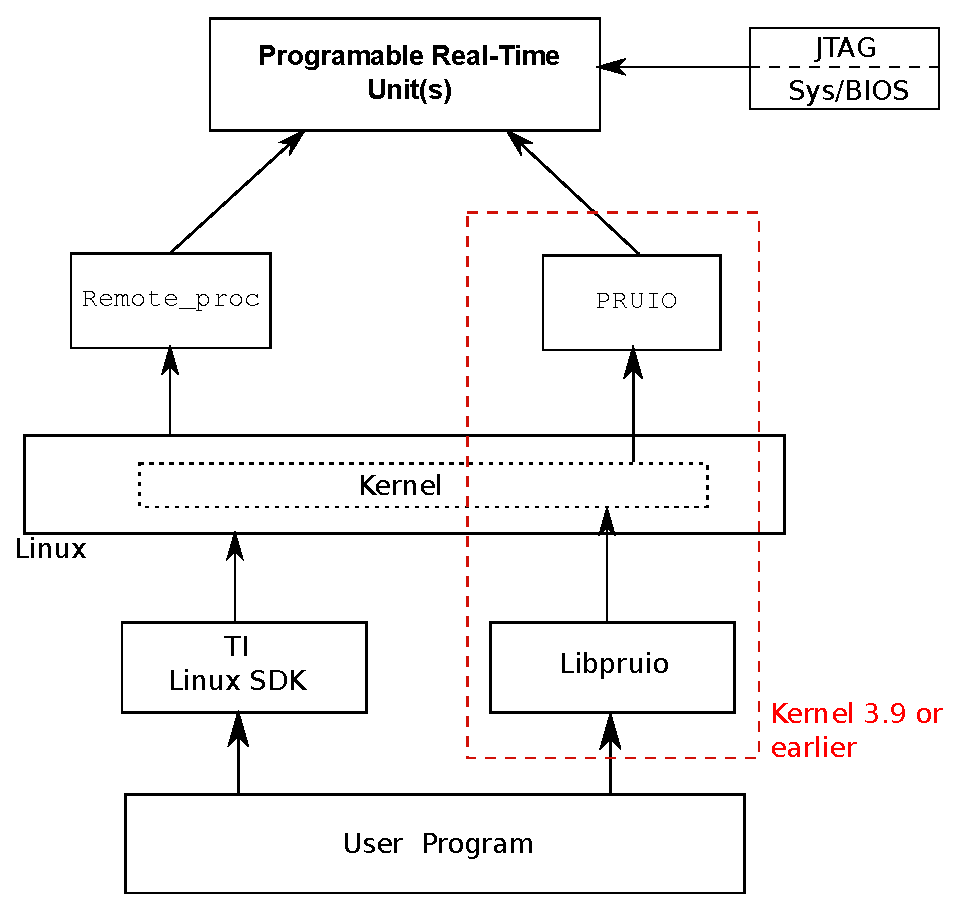
\includegraphics[width=\textwidth]{fig/PRU_config.eps}
	\caption{PRU Configuration Methods}
	\label{fig:pru_config}
\end{figure}

\subsection{PRU Configuration}
There are several way to configure PRUs, depending upon the kernel version, Operating System and the mode of connection.
\begin{enumerate}
	\item PRUIO - PASM 
	\item Remote\_Proc
	\item Direct firmware loading via JTAG
\end{enumerate}

A visual overview of different way of accessing PRUs is show in Fig: \ref{fig:pru_config}.
\subsubsection{PRUIO}
 For Kernel version older then 3.9 PRUIO kernel module is used which uses a Device Tree Overlay. Device trees are a way to describe Hardware in system, their memory address, their port number or there function. A good example of it would be how UART is described in the system. Device tree enables addition of new hardware in run-time from User Space, in the kernel architecture. 
 
 Usually "Board File" is used in kernel package to describe a hardware of specific embedded system, but given the huge number of ever increasing ARM based devices it was impossible to incorporate all the boards' file in to main Kernel. So Linus Torvalds \cite{DThist} suggested the use of DT , to simplify the kernel maintenance and up-keeping while providing complete flexibility to describe their processor (something that was already being done by PowerPC manufacturers). So, usage of kernel module and Device Tree enables enables us to configure PRUs and use them. it maps PRU's register memory address to our use space addresses and enables direct access to them. 
 
 A library  called as "libpruio" \cite{libpruio} is used here, for convenience and rapid development. The library provides C and FreeBasic API's for accessing and configuring ADC, GPIO and PWM modules. It uses converts user C code to Assembly Language via PASM and uploads it to the respective PRUs. A detailed explanation along with program listing is given in Appendix-1.
 
 \subsubsection{Remote\_Proc}
 Modern SoCs have multiple processors and processor cores on them in asymmetric multiprocessing (AMP) configuration. which may be running different instances  of operating system, whether it's Linux or any other flavor of real-time OS  . So to enable single kernel to control all those remote processors while abstracting hardware differences and there by reducing the duplication of code \textit{Remote Processor Framework} is used \cite{remoteproc}.
 
 Here in case of AM3358, Remoteproc acts as a framework that allows the ARM host processor(s) to load firmware into PRU cores, start the PRU cores, stop the PRU cores, and configure resources that the PRUs might need during their execution (such as configuring the PRUSS INTC module and providing shared buffers in DDR memory for message passing).

\subsubsection{Direct Loading}
TI provides different development mediums for it's products, For  AM335x also, there existed - Sys/BIOS support, TI Starterware support and Ti Processors-SDK support. out of which Sys/Bios ad Starterware are a non-OS solution which posses bare minimum driver support in form of modules, which is very useful in rapid development and due to no OS, latency was brought down to bare minimum.
\begin{figure}[h]
	\centering
	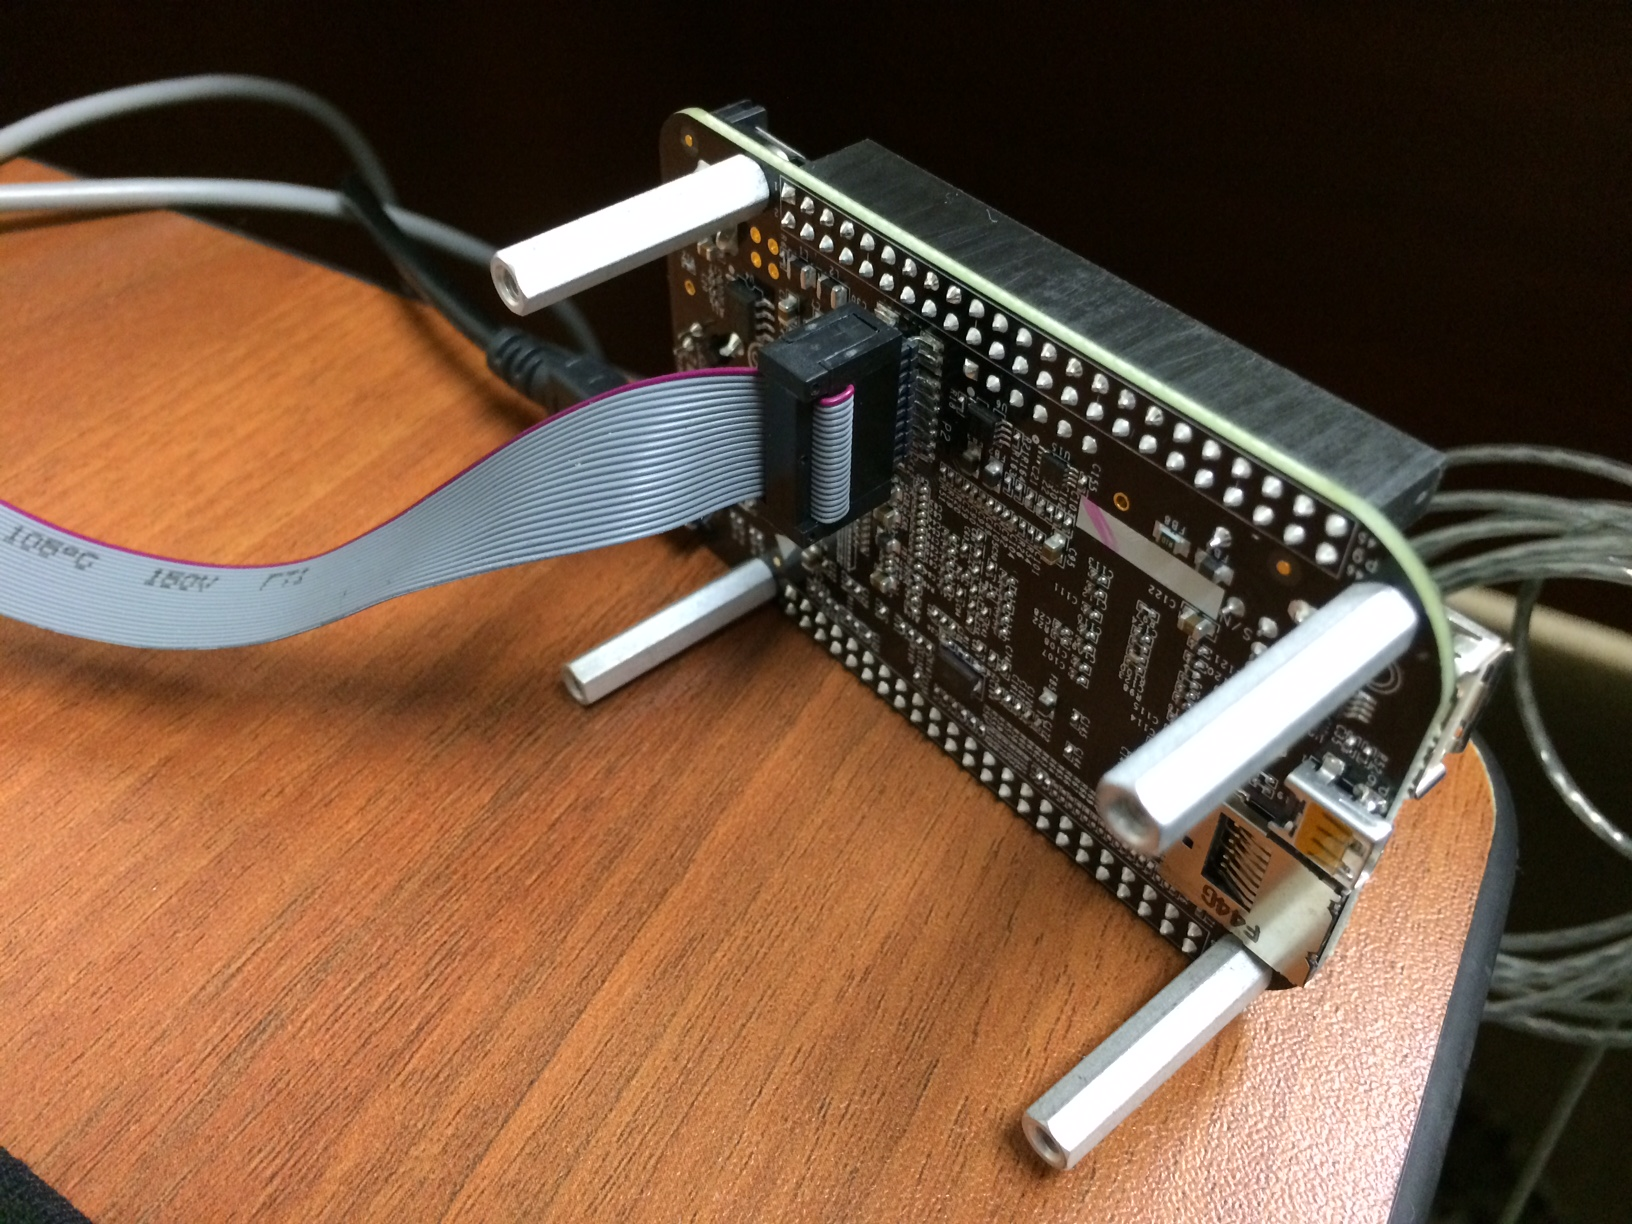
\includegraphics[width=\textwidth/2]{fig/bbb_jtag.jpg}
	\caption{A BeagleBone connected Via Ti's Hawk JTAG}
\end{figure}

Efforts were made to utilize Sys/Bios initially for the project but it had become obsolete and was being phased out which resulted into poor support for relatively newer processor like AM3358. Then efforts were made for using TI-Processor SDK as well, but it required a special ARM \texttt{TMDSEMU100v2U-20T} JTAG-extension header-connector which was not available and hence had to be dismissed. But in principal if one possesses the JTAG, TI-processors SDK can be a very competitive implementation compared to a Linux based implementation, due to real-time capability, direct access to PRU and optimized device drivers by Ti itself.


\subsection{Time stamp, GPS interfacing and Data Processing }
As seen in the previous section, data is read in chunks each chunk has 768 samples which consists of 128 samples from all 6 channels. This makes it more convenient to handle and process the data. Using GPS for time reference was aimed but due to hardware interfacing issues, GPS could not be interfaced instead Network Time Protocol (NTP) is being used for time-keeping. Time stamp for each frame is stored on the first sample of the frame written to the buffer.

\begin{itemize}
	\item DFT window of 3 cycle 384 is chosen for better frequency resolution, and then hamming window is applied to smooth out the samples.
	\item After dot product of samples with hamming constant, DFT is done and frequency is extracted from the beans. 
	\item Frequency resolution is of 0.5 Hz is aimed.
	\item After extracting the frequency, amplitude and angle is extracted by computing the power of all the frequency beans and averaging it and from the \texttt{arctan} of the complex result.
\end{itemize} 

\subsection{Communication}

After DFT is calculated we have the necessary information to send. Structure of the frame depends upon the configuration and specification of the PMU. Hence as per standards a configuration frames should be communicated by PMU to PDC, which lists following things:
\begin{enumerate}
	\item Time Format 
	\item Number of phasors
	\item Format of the phasor (rect or polar)
	\item Frequency
	\item Number of digital status, if any
	\item Error Bit
\end{enumerate}

The frame configuration used by our device is as show below:
\begin{itemize}
	\item TimeTag (8 byte)
	\item 6 phasor entity (6 * 8 bytes)
	\item Frequency (8 Bytes)
\end{itemize}
Once the device turns ON, it PMU establishes a communication to the PDC, by communicating a acknowledgment string once that is communicated PMU starts sending the data to the PDC. Currently PDC is implemented by us, which receives the data over ethernet via TCP/IP, separates each information from frames and writes it to the file. For evaluation purposes the communication delay, sampling delays and reporting time are computed. This is done by computing the time difference between two frame received, by measuring time difference between two time tags of consecutive data frames and by measuring the time taken for the data packets to be received. 

\section{Challenges Faced}
There were several challenges faced and solved which are worth mentioning for others who might embark on this path and face it

\begin{itemize}
	\item GPS module interfacing
	
	NavSync CW-12 TIM GPS module was chosen to provide time to the device. It was connected to the GPS antenna, power was provided and sometimes it lock to 3 Satellites but it fails to get interfaced via serial ports. It has UART \texttt{RxD} and \texttt{TxD} , \texttt{GND} and \texttt{Vcc} pin out.  For configuring it a utility called \textit{WinOnCore} is provided for Windows bases systems. GPS module's UART is connected to PC via FTDI R232L serial to serial convert IC and sends messages to the utility. The problem is while grounds of both system (GPS receiver and PC) are separate WinOnCore fails to communicate with the module but upon looking in "serial terminal" some random message are being thrown by the module. Yet, the moment ground of device is connected to the ground of PC, even those messages stop working. This is a very unusual behavior, Efforts with different power supply, with a new GPS receiver, with different USB to serial converter but all efforts are futile yet.
	
	\item DFT computation Time 
	PMU's DFT requirements are not so complicated and the computational power at hand is also limited hence simple brute force DFT is tried. but it was taking huge time to compute on ARM processor. Initial latency observed was as high as $4.23 ~ms$/channel. Which was optimized by implementing \texttt{look-up tables} and by removing the \texttt{divisions} and putting multiply instead. Now each DFT operation typically  takes 240 to 400 $\mu s$. 
	
	\item Overlapping ADC samples 
	

\end{itemize}